\documentclass{beamer}
\usetheme[subsectionpage=progressbar,block=fill]{metropolis}

\usepackage{svg}

\title{Dezentrale Vernetzung über den Dächern}
\date{16.07.2019}
\author{Freifunk Franken}
\begin{document}
	\maketitle
	\begin{frame}{Übersicht}
		\tableofcontents
	\end{frame}

	\section{Hotspots}
	\begin{frame}[plain]{Hotspots in Nürnberg}
		\centering
		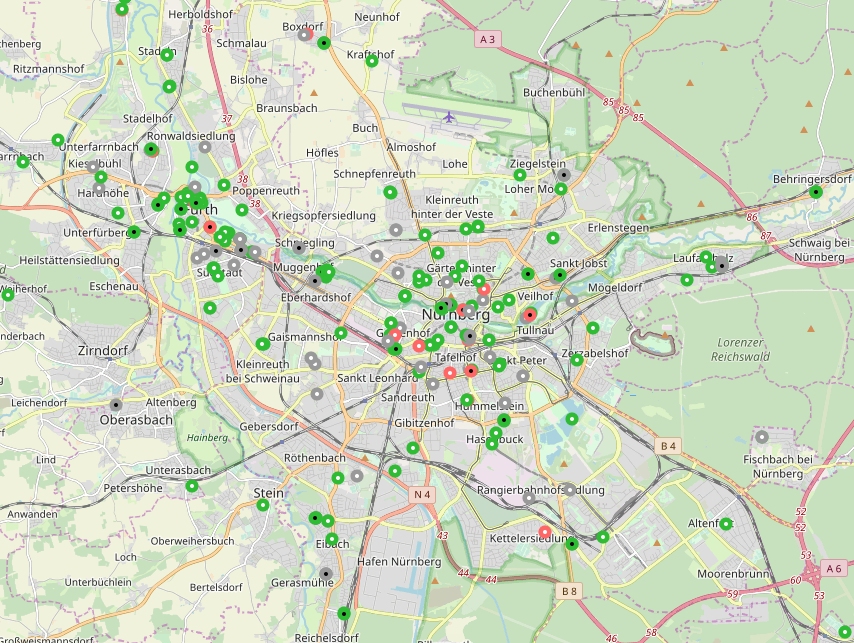
\includegraphics[width=0.94\textwidth]{media/hotspots.png}
	\end{frame}
	\begin{frame}{Freifunk Hotspots}
		\begin{block}{Hotspots}
			\begin{itemize}
				\item Bekannteste Form von Freifunk
				\item Auch in Nürnberg/Franken
			\end{itemize}
		\end{block}
		\vspace{1em}
		\pause
		\begin{block}{Teilen des eigenen Internetanschlusses}
			\begin{itemize}
				\item Router mit Freifunk Firmware
				\item Tunnel zu Freifunk Server
				\item Umgehung rechtlicher Probleme
			\end{itemize}
		\end{block}
	\end{frame}

	%\subsection{Vernetzung per Mesh}
	\begin{frame}{Vernetzen per Mesh}
		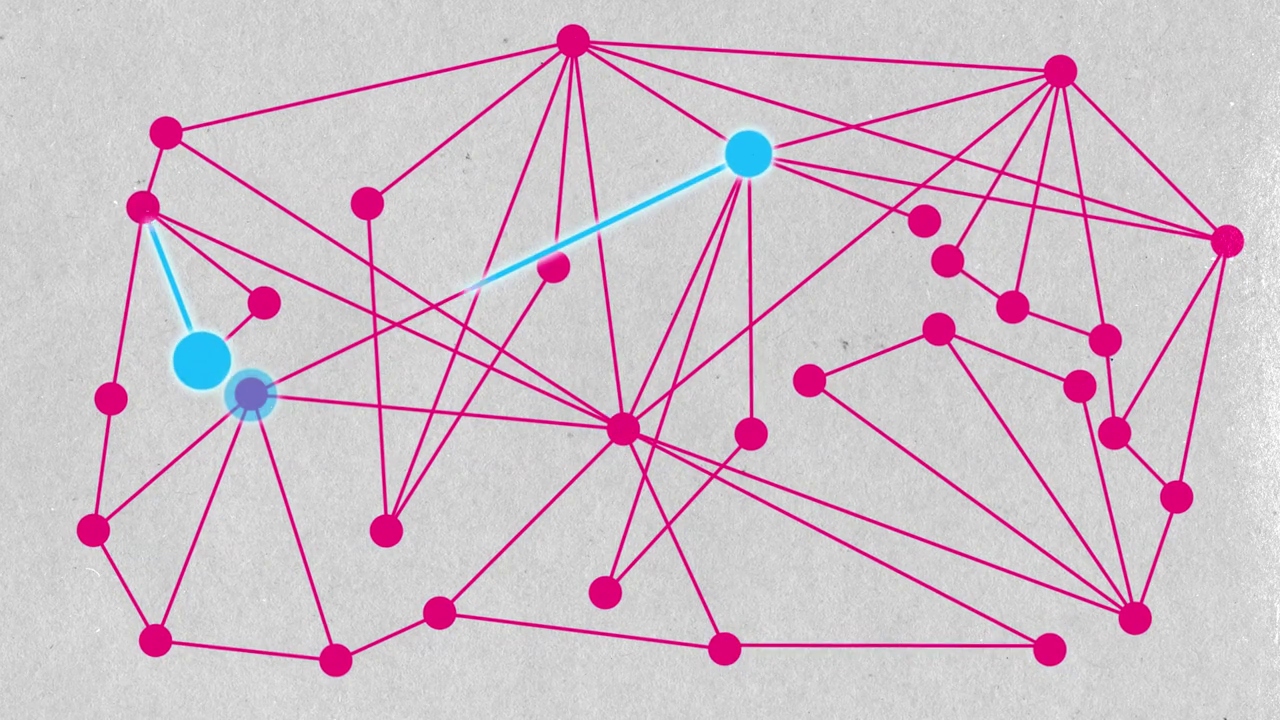
\includegraphics[width=\textwidth]{media/mesh2.png}
	\end{frame}

	%\subsection{Entwicklung}
	\begin{frame}{Entwicklung}
		\begin{block}{Hotspots}
			\begin{itemize}
				\item Immer mehr
				\item Teilweise in Kooperation mit Städten
			\end{itemize}
		\end{block}
		\vspace{1em}
		\pause
		\begin{block}{Backend}
			\begin{itemize}
				\item Wenig Interaktion zwischen Freifunkern
				\item Mesh eher selten und extrem langsam
				\item Klappt nicht so, wie man sich das dachte
			\end{itemize}
		\end{block}
	\end{frame}


	\section{Dezentrale Vernetzung}
	\begin{frame}[plain,standout]
		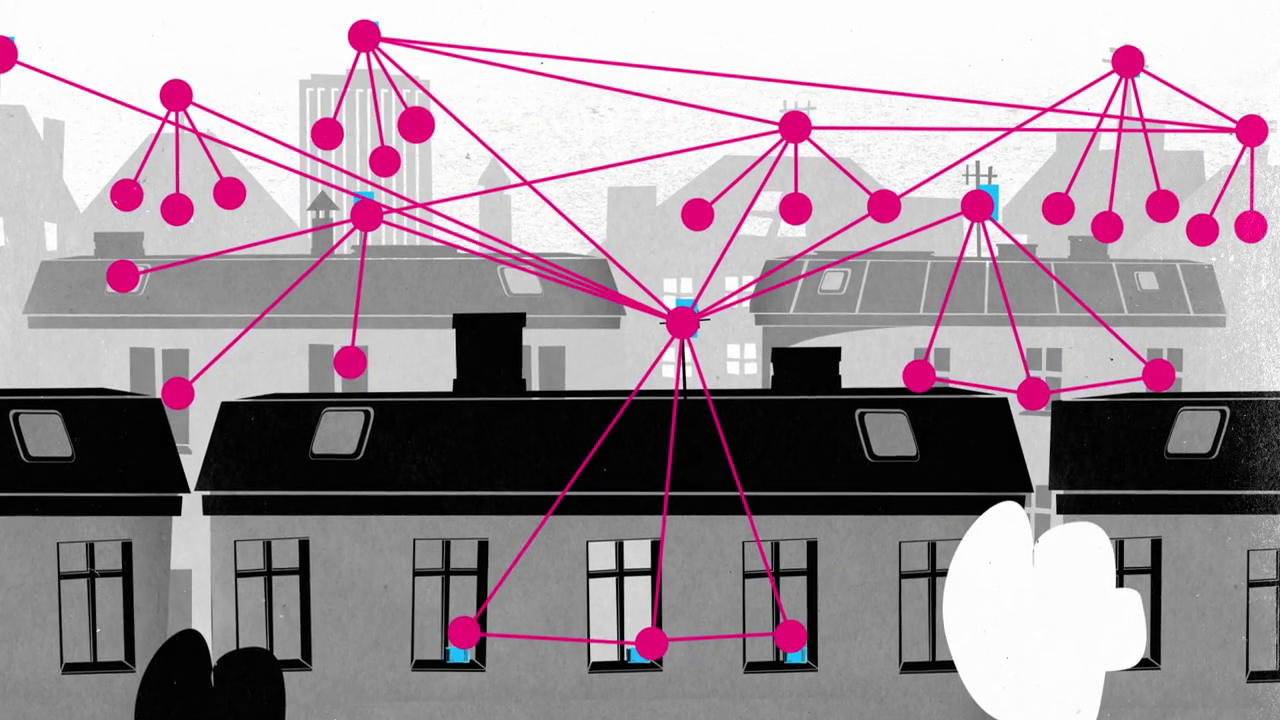
\includegraphics[width=\framewidth]{media/dachzudach.png}
	\end{frame}
	\begin{frame}[plain,standout]
		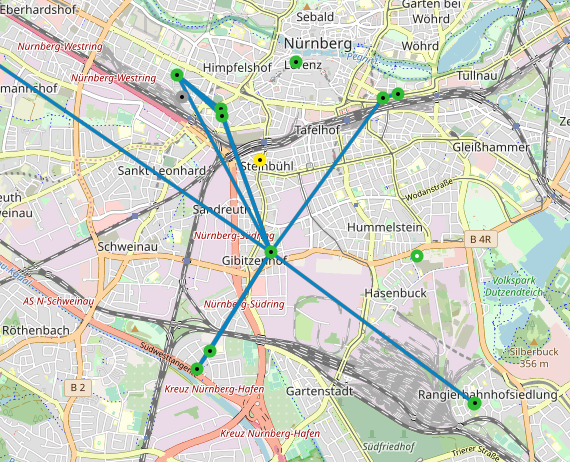
\includegraphics[width=0.95\framewidth]{media/rf_nbg.png}
	\end{frame}
	\begin{frame}[plain,standout]
		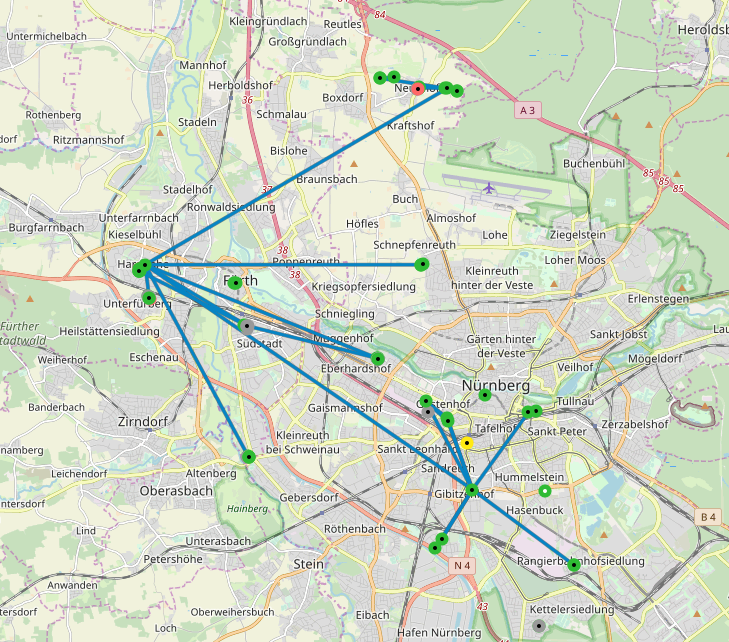
\includegraphics[width=0.95\framewidth]{media/rf_nbgfue.png}
	\end{frame}

	\begin{frame}{Pico-Peering Agreement}
		\textbf{Regelwerk, über grundsätzliche Eigenschaften des Freifunks}

		\begin{enumerate}
			\item Freier Transit
			\item Offene Kommunikation
			\item Keine Garantie (Haftungsausschluss)
			\item Nutzungsbestimmungen
			\item Lokale (individuelle) Zusätze
		\end{enumerate}
	\end{frame}

	\section{Tiefere Einblicke}
	\begin{frame}{IPv6}
	\end{frame}

	\begin{frame}{BGP}
	\end{frame}

	\begin{frame}{N-IX}
	\end{frame}
\end{document}
